\section{ASM Definition of Subject Execution}

\setminted{fontsize=\small}
\setmintedinline{fontsize=\normalsize,breaklines}

% NOTE: DRAFT WOLSKIA

This section provides a reduced overview of the ASM semantics given in Appendix~\ref{CoreASM-Reference-Implementation}.

The goal of this section is to provide a minimal set of reduced rules to establish a foundation to understand the ASM semantics,
leaving out certain features and implementation details.
It is therefore just an informal introduction to the topic.

Please note the conceptual differences between the interpreter semantics and the owl structure, presented in \ref{CoreASM-Reference-Implementation-Differences-OWL-Model}.
Most importantly, the interpreter semantics for interaction support only "IP strategy blocking".

simplifications for this chapter:
\begin{itemize}
	\item no Observer support => no execution state, no state priorities => Cancel not required
	\item limited scope to InternalAction, Send, Receive, CallMacro, ModalSplit/ModalJoin, End => no VarMan, Cancel, SelectAgents, Tau
	\item discuss: proper-termination and CloseIP/OpenIP are motivated from interaction soundness. include? mention? hard-exclude (remove references from code)?
	\item no KillBehavior (although recursive macros and reservation messages). therefore this will not be sound - but a bit less complicated
\end{itemize}


\subsection{Architecture}

\begin{figure}[htbp]
	\centering
	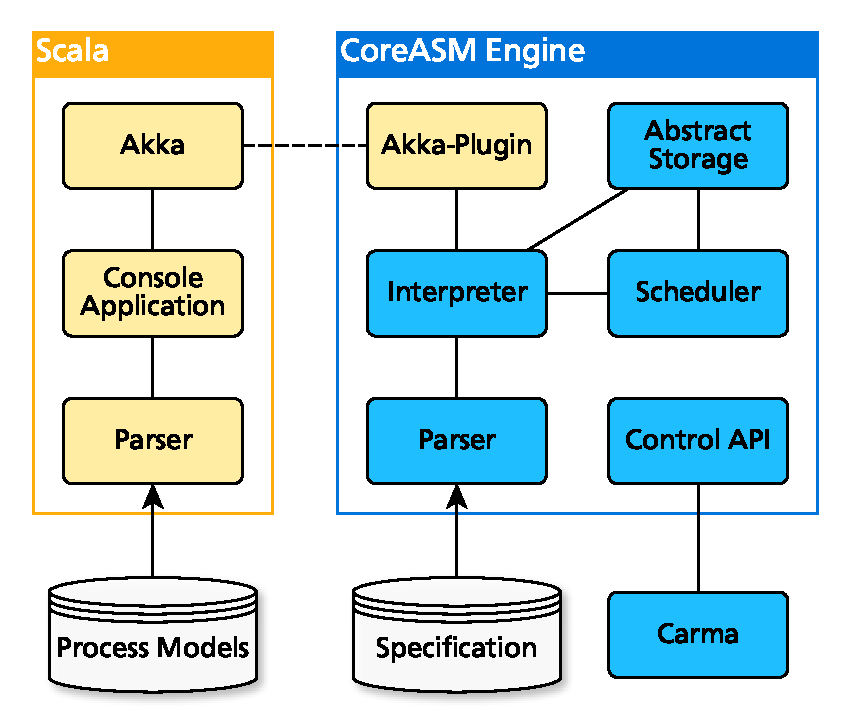
\includegraphics[width=0.7\linewidth]{Figures/CoreASM/ArchitekturKonsoleCoreASM}
  \caption{Runtime environments and system components. The blue (dark background) components are part of the Java based CoreASM Engine. The yellow (light background) components are developed by us by using the Scala programming language \citep{ecole_polytechnique_federale_scala_2019} and the Akka actor library \citep{lightbend_inc_akka_2019}.}
  \label{fig:coreasm_architecture}
\end{figure}

The overall architecture is shown in figure~\ref{fig:coreasm_architecture} and consists on the top level of
a console application as user interface and the CoreASM engine.
Both high level components are running in parallel in separate Java Virtual Machine processes.
The locally stored specification file includes an ASM specification of asynchronous multi-agent ASMs, executing each Subject by one ASM-agent each.


The CoreASM engine parses the specification file and executes the rules in the interpreter
in cooperation with the abstract storage and the scheduler.
The abstract storage stores the state of the ASM and is also used to support
TurboASMs and their submachine states.

The scheduler is used to support asynchronous multi-agent ASMs; with
the \textit{default} scheduling policy it selects
a random subset of the running ASM agents and calls the
interpreter for the parallel evaluation of their main rules.
If the resultant update sets
are consistent they are applied in the abstract storage, otherwise the scheduler
selects a different subset of the running ASM agents for a re-evaluation.
Supplementary the \textit{onebyone} scheduling policy can be used to evaluate
only a single agent per step and the \textit{allfirst} policy can be used
to attempt to evaluate all agents at once before falling back
to the default scheduling policy in case of inconsistencies.
We use the \textit{allfirst} scheduling policy in our work for performance reasons
but could use the \textit{default} policy as well.

The Carma application is a simple Java application provided by the CoreASM framework
to allow the usage of the CoreASM engine as standalone application in a command line.

The console application is developed in Scala.
A user can load, start and execute locally stored S-BPM Process Models with it.
The interaction between the console application and the CoreASM engine is realized by Akka actors.
The Akka actor of the engine has full read and write access to all CoreASM functions by using a Plug-In interface.




\subsection{Foundation}

The interpreter uses asynchronous multi-agent Turbo ASMs.
It supports the concurrent execution of multiple process models and multiple instances of each process model.
Each instance has a unique \textit{ProcessInstanceID} (short: \asminline{PI}) assigned.
Within a process instance multiple instances of a subject can occur (MultiSubject concept).
Each subject instance has an agent assigned, to distinguish the subject instances.
This agent is identified by it name.
We therefore identify a subject instance by the tuple (Process~Model~ID, Process~Instance~ID, Subject~ID, Agent~Name).
This tuple is called \textit{Channel} (short: \asminline{ch}), as it used in the mobility of channels concept in order to support distributed communication patterns.

In the interpreter, each subject instance has an ASM Agent assigned, that keeps track of its current state,
where we mean state in the sense of which subject data is present, the content of the inputpool queues and also the active SBD states.
This state is stored in ASM functions and assigned to the \textit{Channel}.

\begin{listing}[htbp]
\begin{minted}{lexer.py:CoreASMLexer -x}
// ASM Agent -> Channel
function channelFor : Agents -> LIST

derived processIDFor(a)       = processIDOf(channelFor(a))
derived processInstanceFor(a) = processInstanceOf(channelFor(a))
derived subjectIDFor(a)       = subjectIDOf(channelFor(a))
derived agentFor(a)           = agentOf(channelFor(a))

derived processIDOf(ch)       = nth(ch, 1)
derived processInstanceOf(ch) = nth(ch, 2)
derived subjectIDOf(ch)       = nth(ch, 3)
derived agentOf(ch)           = nth(ch, 4)
\end{minted}
\caption{Channel definitions}
\label{lst:shortasm:channelFor}
\end{listing}

In the function \asminline{channelFor} the assignment from the ASM Agents to their \textit{Channels} is stored.
The derived functions are used to lookup certain tuple elements of the channel.\\

% NOTE: StartProcess and StartASMAgent left out intentionally

% Subject Data

Analogous to programming languages we call Subject Data \textit{Variables}.
Their scope is either bound to a Subject or a Macro Instance and can only be
accessed by the Subject. Variables are identified by their name and have an
explicit data type and a value.

Variables are stored in the \asminline{variable} function which maps from
the Subject's Channel, the scoped Macro Instance~ID and the Variable's name to
a pair of the data type and value. For Variables that are not scoped to a Macro
Instance, and are therefore accessible for any state in any Macro Instance of
the Subject, the unused Macro Instance~ID~0 is used.

The function \asminline{variableDefined} is used to keep track of Variables
that are in use, so that their content can be reset upon the termination of a
Macro Instance or the Subject, respectively.


\begin{listing}[htbp]
\begin{minted}{lexer.py:CoreASMLexer -x}
// Channel * macroInstanceNumber * varname -> [vartype, content]
function variable : LIST * NUMBER * STRING -> LIST

// Channel -> Set[(macroInstanceNumber, varname)]
function variableDefined : LIST -> SET
\end{minted}
\caption{variable}
\label{lst:shortasm:variable}
\end{listing}




\subsection{Interaction Definitions}\label{sec:InteractionDefinitions}

We implement the interaction between Subjects as asynchronous Message exchange.
Messages are placed into the Inputpool of the receiver where they are then retrieved from when the receiver is in a Receive state.


\subsubsection{Messages}\label{sec:messages}

The message content consists of the actual payload and its data type. As this
reference implementation is intended only for an abstract process execution we abstract
the payload / business objects to be just a text given as string.

For the communication with MultiSubjects, i.e. sending the same Message to
multiple Agents of one Subject, we use an \textit{all-or-none} strategy. This
is accomplished by separating the sending of a Message into two phases: first
a reservation Message is placed at each receiver into the Inputpool.
Only after all reservations could be placed they are then replaced with the
actual Message.

\subsubsection{Inputpool}\label{sec:Inputpool}

The Inputpool is structured into multiple FIFO queues per Subject~ID of the sender, the Messagetype and the CorrelationID.

The Inputpool can be limited to allow a maximum number of Messages and
reservations per sender Subject~ID and Messagetype; in case the Inputpool Limit is
reached no additional reservation can be placed. To support the proper
termination of a Subject a specific queue (and also the complete Inputpool)
can be closed, in which case no additional reservation can be placed into it,
too.

\begin{listing}[htbp]
\begin{minted}[escapeinside=~~]{lexer.py:CoreASMLexer -x}
// Channel * senderSubjID * msgType * correlationID
//   -> [msg1, msg2, ~\ldots~]
function inputPool : LIST * STRING * STRING * NUMBER -> LIST

/* stores all locations where an inputPool was defined */
// Channel -> {[senderSubjID, msgType, correlationID], ~\ldots~}
function inputPoolDefined : LIST -> SET

// Channel * senderSubjID * msgType * correlationID
function inputPoolClosed : LIST * STRING * STRING * NUMBER
  -> BOOLEAN
\end{minted}
\caption{inputPool}
\label{lst:shortasm:inputPool}
\end{listing}


The queues of the Inputpool are stored in the \asminline{inputPool} function.
The function \asminline{inputPoolDefined} is used to keep track of the
locations of the queues that are in use, so that their content can be checked
upon termination. The function \asminline{inputPoolClosed} is used to store
whether a queue is closed. The special location
\asminline{inputPoolClosed(ch, undef, undef, undef)} is used to
store whether the complete Inputpool is closed.

We define the function \asminline{derived availableMessages(receiverChannel, senderSubjectID, msgType, ipCorrelationID)} to return the
Messages from the location \asminline{inputPool(receiverChannel,
senderSubjectID, msgType, ipCorrelationID)} that can be received, i.e. that it
filters out reservations and reduces Messages from the same sender to only
the oldest one.

\subsection{Subject Behavior}


As depicted in figure~\ref{fig:MainSBPM components}, a Subject Behavior consists at least of one \textit{Main Macro}
and might have an arbitrary number of minor Macros, called \textit{Additional Macros}.

\begin{listing}[htbp]
\begin{minted}{lexer.py:CoreASMLexer -x}
rule SubjectBehavior =
  MacroBehavior(1)
\end{minted}
\caption{SubjectBehavior}
\label{lst:shortasm:SubjectBehavior}
\end{listing}

% Macro Behavior

% NOTE: extemely shortened: no execution state => no remainingStates


The \asminline{MacroBehavior} rule controls the evaluation of all active
states for the given Macro Instance~ID~\asminline{MI}.


\begin{listing}[htbp]
\begin{minted}{lexer.py:CoreASMLexer -x}
rule MacroBehavior(MI) =
  let ch = channelFor(self) in
  choose stateNumber in activeStates(ch, MI) do
    Behavior(MI, stateNumber)
\end{minted}
\caption{MacroBehavior}
\label{lst:shortasm:MacroBehavior}
\end{listing}

From that list a state \asminline{stateNumber} is chosen to be evaluated with the \asminline{Behavior} rule.

% State


The evaluation of a state is structured into three main phases: initialization,
the state function and an optional transition behavior.

The state function is responsible for the selection of an outgoing transition and
has to supervise the Timeout. It also has to enable and disable its outgoing
transitions, meaning that transitions can be available depending on some dynamic state,
for example whether a certain Message is present in the Inputpool.
Usually the outgoing transition will be selected by the environment, however with
auto-transitions it is possible that such an transition is automatically selected as soon
as it becomes enabled and as long as there are no other transitions to select from.


\begin{listing}[htbp]
\begin{minted}{lexer.py:CoreASMLexer -x}
rule Behavior(MI, currentStateNumber) =
 let s = currentStateNumber,
    ch = channelFor(self) in
  if (initializedState(ch, MI, s) != true) then
    StartState(MI, s)
  else if (abortState(MI, s) = true) then
    AbortState(MI, s)
  else if (completed(ch, MI, s) != true) then
    Perform(MI, s)
  else if (initializedSelectedTransition(ch, MI, s) != true) then
    StartSelectedTransition(MI, s)
  else
   let t = selectedTransition(ch, MI, s) in
    if (transitionCompleted(ch, MI, t) != true) then
      PerformTransition(MI, s, t)
    else
      Proceed(MI, s, targetStateNumber(processIDFor(self), t))
\end{minted}
\caption{Behavior}
\label{lst:shortasm:Behavior}
\end{listing}


In the beginning the \asminline{Behavior} rule initializes the state with the
\asminline{StartState} rule, which will set \asminline{initializedState} to
\asminline{true}. If the function should not be aborted the \asminline{Perform}
rule calls the state behavior of the underlying function until it is
\asminline{completed}.
In the next phase the selected transition will be initialized by the
\asminline{StartSelectedTransition} rule and the transition behavior will be performed with
the \asminline{PerformTransition} rule until it is completed as well. As last step
the \asminline{Proceed} rule removes the current state and adds the selected
transition's target state.

%---

The environment has full read access to all functions of this semantics and knows
therefore each running Subject, their Macro Instances and their active states.

To define a homogeneous interface between the Function semantics and the environment we
define the function \asminline{wantInput} to be written by an Function when it
requires an external input, for example if an outgoing transition has to be chosen.



\begin{listing}[htbp]
\begin{minted}{lexer.py:CoreASMLexer -x}
// Channel * MacroInstanceNumber * StateNumber -> Set[String]
function wantInput : LIST * NUMBER * NUMBER -> SET
\end{minted}
\caption{wantInput}
\label{lst:shortasm:wantInput}
\end{listing}


This function is read by our console application for all active states
to present the user a list of possible decisions that can be made.

The environment then writes its external input in a corresponding function, for
example for a transition decision into the \asminline{selectedTransition} function, and
clears the \asminline{wantInput} function of that state.

The \asminline{SelectTransition} rule adds the \asminline{"TransitionDecision"}
requirement into the \asminline{wantInput} function.


\begin{listing}[htbp]
\begin{minted}{lexer.py:CoreASMLexer -x}
rule SelectTransition(MI, currentStateNumber) =
  let ch = channelFor(self),
       s = currentStateNumber in
  if (|outgoingEnabledTransitions(ch, MI, s)| = 0) then
    skip // BLOCKED: none to select
  else if (not(contains(wantInput(ch, MI, s),
                        "TransitionDecision"))) then
    add "TransitionDecision" to wantInput(ch, MI, s)
  else
    skip // waiting for selectedTransition
\end{minted}
\caption{SelectTransition}
\label{lst:shortasm:SelectTransition}
\end{listing}


If the \asminline{wantInput} function already contains the
\asminline{"TransitionDecision"} requirement nothing needs to be done and another
state can be evaluated by the \asminline{MacroBehavior} rule.
The same applies if there are no outgoing transitions enabled.
Otherwise the requirement is added to the \asminline{wantInput} function.


\subsection{Internal Action}


The \emph{Internal Action} is used to model DoStates, Subject-internal activities and decisions.
It is labeled with a textual description of the activity that the Agent should perform.
The outgoing transitions are labeled with a textual description of the possible execution results.
Since the activity is performed outside of the interpreter all outgoing transitions are enabled from the beginning on and no transition rule has to be defined.
Therefore the state function only consists of the timeout check and transition selection.


\begin{listing}[htbp]
\begin{minted}{lexer.py:CoreASMLexer -x}
rule StartInternalAction(MI, currentStateNumber) = {
  StartTimeout(MI, currentStateNumber)

  EnableAllTransitions(MI, currentStateNumber)
}
\end{minted}
\caption{StartInternalAction}
\label{lst:shortasm:StartInternalAction}
\end{listing}



The initialization of the InternalAction starts the Timeout and enables all
outgoing transitions.


\begin{listing}[htbp]
\begin{minted}{lexer.py:CoreASMLexer -x}
rule PerformInternalAction(MI, currentStateNumber) =
  let ch = channelFor(self),
       s = currentStateNumber in
    if (shouldTimeout(ch, MI, s) = true) then {
      SetCompleted(MI, s)
      ActivateTimeout(MI, s)
    }
    else if (selectedTransition(ch, MI, s) != undef) then
      SetCompleted(MI, s)
    else
      SelectTransition(MI, s)
\end{minted}
\caption{PerformInternalAction}
\label{lst:shortasm:PerformInternalAction}
\end{listing}


The state function checks if a Timeout should be activated; otherwise the
\asminline{SelectTransition} rule is called until the \asminline{selectedTransition} function has
been set.




\subsection{Send Function}


The Send Function sends a Message. Disregarding the optional Timeout and Cancel
transitions it must have exactly one outgoing transition which has to have parameters that
define at least the Messagetype and the receiver's Subject~ID.

We use an \textit{all-or-none} strategy to send Messages to MultiSubjects,
which means that the actual Message is only send when all receivers are able
to store it in their Inputpool. Therefore the Send Function is structured into
two phases: in the first phase, realized as state function, reservation Messages
are placed and in the second phase, realized as transition function, these reservations
are replaced with the actual Message.

To place a reservation in a receiver's Inputpool there must be space available
in the corresponding queue and the receiver must not be
\textit{non-proper} terminated.


\begin{listing}[htbp]
\begin{minted}{lexer.py:CoreASMLexer -x}
// Channel * MacroInstanceNumber * StateNumber -> Set[Messages]
function receivedMessages : LIST * NUMBER * NUMBER -> SET

// Channel * MacroInstanceNumber * StateNumber -> Set[Channel]
function receivers : LIST * NUMBER * NUMBER -> SET

// Channel * MacroInstanceNumber * StateNumber
function messageContent       : LIST * NUMBER * NUMBER -> LIST
function messageCorrelationID : LIST * NUMBER * NUMBER -> NUMBER
function messageReceiverCorrelationID : LIST * NUMBER * NUMBER
  -> NUMBER

// Channel * MacroInstanceNumber * StateNumber -> Set[Channel]
function reservationsDone : LIST * NUMBER * NUMBER -> SET

function nextCorrelationID : -> NUMBER
function nextCorrelationIDUsedBy : NUMBER -> Agents
\end{minted}
\caption{receivedMessages}
\label{lst:shortasm:receivedMessages}
\end{listing}


The Send Function stores the message content it has to send in the
\asminline{messageContent} function. The \asminline{receivers} function is
used to store the required receivers. When a reservation message has been
placed at a receiver its Channel is added to the \asminline{reservationsDone}
function.

The global function \asminline{nextCorrelationID} is used to increment
CorrelationIDs. To ensure the uniqueness of a CorrelationID the
\asminline{nextCorrelationIDUsedBy} function is used to store the ASM agent
that used the given CorrelationIDs.


\begin{listing}[htbp]
\begin{minted}{lexer.py:CoreASMLexer -x}
rule StartSend(MI, currentStateNumber) =
  let ch = channelFor(self),
     pID = processIDFor(self),
       s = currentStateNumber in
  // there must be exactly one transition
  let  t = first_outgoingNormalTransition(pID, s) in {
    receivers(ch, MI, s) := undef
    reservationsDone(ch, MI, s) := {}
    let mcVName = messageContentVar(pID, t) in
      messageContent(ch, MI, s) := loadVar(MI, mcVName)

    // generate new CorrelationID now, it will be stored
    // in a Variable once the message(s) are send
    let cIDVName = messageNewCorrelationVar(pID, t) in
      if (cIDVName != undef and cIDVName != "") then {
        messageCorrelationID(ch, MI, s) := nextCorrelationID
        nextCorrelationID := nextCorrelationID + 1
        // ensure no other agent uses this same correlationID
        nextCorrelationIDUsedBy(nextCorrelationID) := self
      }
      else
        messageCorrelationID(ch, MI, s) := 0

    // load receiver IP CorrelationID now, to avoid
    // influences of any changes of that variable
    let cIDVName = messageWithCorrelationVar(pID, t) in
    let cID = loadCorrelationID(MI, cIDVName) in
      messageReceiverCorrelationID(ch, MI, s) := cID
  }
\end{minted}
\caption{StartSend}
\label{lst:shortasm:StartSend}
\end{listing}


The initialization of the Send Function resets / initializes the \asminline{receivers} and
\asminline{reservationsDone} functions.
If the communication transition has a \asminline{messageContentVar} parameter given the
content of that Variable is loaded and stored in the \asminline{messageContent}
function. If it has a \asminline{messageNewCorrelationVar} parameter given
a new CorrelationID is created and stored in the \asminline{messageCorrelationID} function.
It will be stored in the Variable after the messages have been send.
If the message that will be send correlates to a previous message from the receiver
the CorrelationID from the Variable in \asminline{messageWithCorrelationVar} will be loaded
so that the message is stored in the corresponding inputpool queue of the receiver.


\begin{listing}[htbp]
\begin{minted}{lexer.py:CoreASMLexer -x}
rule PerformSend(MI, currentStateNumber) =
  let ch = channelFor(self),
       s = currentStateNumber in
  if (receivers(ch, MI, s) = undef) then
    SelectReceivers(MI, s)
  else if (messageContent(ch, MI, s) = undef) then
    SetMessageContent(MI, s)
  else if (startTime(ch, MI, s) = undef) then
    StartTimeout(MI, s)
  else if (|receivers(ch, MI, s)| =
           |reservationsDone(ch, MI, s)|) then
    TryCompletePerformSend(MI, s)
  else if (shouldTimeout(ch, MI, s) = true) then {
    SetCompleted(MI, s)
    ActivateTimeout(MI, s)
  }
  else
    DoReservations(MI, s)
\end{minted}
\caption{PerformSend}
\label{lst:shortasm:PerformSend}
\end{listing}


In the state function the \asminline{SelectReceivers} rule is called until
the \asminline{receivers} have been selected. The \asminline{SelectReceivers} rule
interacts with the environment through the Selection and SelectAgent Functions
in order to either select existing Channels from a Variable, given as parameter
on the communication edge, or to select new assignments of Agents for the receiver
Subject.

The Timeout is started only when the \asminline{receivers} and the
\asminline{messageContent} functions are defined. Until all reservations are
placed, and if no Timeout occurs, the \asminline{DoReservations} rule attempts
to place further reservation messages. If all reservations are placed the
\asminline{TryCompletePerformSend} rule completes the state function, depending
on whether no receiver is \textit{non-proper} terminated.


\begin{listing}[htbp]
\begin{minted}{lexer.py:CoreASMLexer -x}
rule SetMessageContent(MI, currentStateNumber) =
  let ch = channelFor(self),
       s = currentStateNumber in
    if not(contains(wantInput(ch, MI, ch),
                    "MessageContentDecision")) then
      add "MessageContentDecision" to wantInput(ch, MI, ch)
    else
      skip // waiting for messageContent
\end{minted}
\caption{SetMessageContent}
\label{lst:shortasm:SetMessageContent}
\end{listing}



The \asminline{SetMessageContent} rule is called if no message content is
given as parameter on the communication transition until the \asminline{messageContent}
function is written by the environment.





\begin{listing}[htbp]
\begin{minted}{lexer.py:CoreASMLexer -x}
// handle all receivers
rule DoReservations(MI, currentStateNumber) =
  let ch = channelFor(self),
       s = currentStateNumber in
  let receiversTodo = (receivers(ch, MI, s) diff
                       reservationsDone(ch, MI, s)) in
  foreach receiver in receiversTodo do
    DoReservation(MI, s, receiver)
\end{minted}
\caption{DoReservations}
\label{lst:shortasm:DoReservations}
\end{listing}



The \asminline{DoReservations} rule iterates over all receivers that did not
already receive a reservation message. The \asminline{DoReservation} rule
then tries to place a reservation message for such receiver.

\begin{listing}[htbp]
\begin{minted}{lexer.py:CoreASMLexer -x}
// handle single reservation
// result true if hasPlacedReservation, adds to reservationsDone
rule DoReservation(MI, currentStateNumber, receiverChannel) =
  if (properTerminated(receiverChannel) = true) then
    let ch = channelFor(self),
       pID = processIDFor(self),
       sID = subjectIDFor(self),
         s = currentStateNumber in
    let Rch = receiverChannel,
       RpID = processIDOf(receiverChannel) in
    let sIDX = searchSenderSubjectID(pID, sID, RpID) in
    let msgCID = messageCorrelationID(ch, MI, s),
        RCID   = messageReceiverCorrelationID(ch, MI, s) in
    // there must be exactly one transition
    let t  = first_outgoingNormalTransition(pID, s) in
    let mT = messageType(pID, t) in
    let resMsg = [ch, mT, {}, msgCID, true] in
      seq
        // prepare receiver IP
        if (inputPool(Rch, sIDX, mT, RCID) = undef) then {
          add [sIDX, mT, RCID] to inputPoolDefined(Rch)
          inputPool(Rch, sIDX, mT, RCID) := []
        }
      next
        if (inputPoolIsClosed(Rch, sIDX, mT, RCID) != true) then
          if (inputPoolGetFreeSpace(Rch, sIDX, mT) > 0) then {
            enqueue resMsg into inputPool(Rch, sIDX, mT, RCID)
            add Rch to reservationsDone(ch, MI, s)
          }
          else
            skip // BLOCKED: no free space!
        else
          skip // BLOCKED: inputPoolIsClosed
  else
    skip // BLOCKED: non-properTerminated
\end{minted}
\caption{DoReservation}
\label{lst:shortasm:DoReservation}
\end{listing}


The \asminline{DoReservation} rule does not try to place a reservation message
if the receiver is \textit{non-proper} terminated. Otherwise it determines
the necessary parameters of the queue to use and builds the reservation message.
To support sending to an External Subject a translation of the sender's original
Subject~ID to the Subject~ID used in the External Process is performed by the
\asminline{searchSenderSubjectID} function.

When the queue at \asminline{inputPool(rCh, xSID, msgType, dstCorr)} was not
created yet a new queue is assigned to that location and remembered in the
\asminline{inputPoolDefined} function on the receiver's side.
If the queue is either closed or full no reservation message can be placed,
otherwise it is enqueued at the end.



\begin{listing}[htbp]
\begin{minted}{lexer.py:CoreASMLexer -x}
rule TryCompletePerformSend(MI, currentStateNumber) =
  let ch = channelFor(self),
     pID = processIDFor(self),
       s = currentStateNumber in
  if (anyNonProperTerminated(receivers(ch, MI, s)) = true) then
    if (shouldTimeout(ch, MI, s) = true) then {
      SetCompleted(MI, s)
      ActivateTimeout(MI, s)
    }
    else
      // BLOCKED: a receiver where a reservation was placed has
      // terminated non-proper in the meantime
      skip
  else {
    // there must be exactly one transition
    let t = first_outgoingNormalTransition(pID, s) in
      selectedTransition(ch, MI, s) := t

    SetCompleted(MI, s)
  }
\end{minted}
\caption{TryCompletePerformSend}
\label{lst:shortasm:TryCompletePerformSend}
\end{listing}


After all reservations could be placed the \asminline{TryCompletePerformSend}
rule has to ensure that no receiver terminated \textit{non-proper} in the
meantime. In that case the Send Function blocks and can only be left by a
Timeout or Cancel transition. Otherwise the state function is completed and the behavior can
continue with the transition function.


\begin{listing}[htbp]
\begin{minted}{lexer.py:CoreASMLexer -x}
rule PerformTransitionSend(MI, currentStateNumber, t) =
  let ch = channelFor(self),
     pID = processIDFor(self),
       s = currentStateNumber in {
    foreach r in reservationsDone(ch, MI, s) do {
      ReplaceReservation(MI, s, r)

      EnsureRunning(r)
    }

    let storeVName = messageStoreReceiverVar(pID, t) in
      if (storeVName != undef and storeVName != "") then
        SetVar(MI, storeVName, "ChannelInformation",
               reservationsDone(ch, MI, s))

    let cIDVName = messageNewCorrelationVar(pID, t) in
      if (cIDVName != undef and cIDVName != "") then
        SetVar(MI, cIDVName, "CorrelationID",
               messageCorrelationID(ch, MI, s))

    SetCompletedTransition(MI, s, t)
  }
\end{minted}
\caption{PerformTransitionSend}
\label{lst:shortasm:PerformTransitionSend}
\end{listing}


The transition function calls the \asminline{ReplaceReservation} rule to replace all
reservations with the actual Message. The \asminline{EnsureRunning} rule
(re)starts a receiver if it is not already running.
If the communication transition has the parameter \asminline{messageStoreReceiverVar} defined
the used receivers of the Message are stored in that Variable.
Also, if the communication transition has the parameter \asminline{messageNewCorrelationVar} defined
the CorrelationID that was created in \asminline{StartSend} and used for the send messages will be stored in the given Variable.


\begin{listing}[htbp]
\begin{minted}{lexer.py:CoreASMLexer -x}
rule ReplaceReservation(MI, currentStateNumber, receiverChannel) =
  let ch = channelFor(self),
     pID = processIDFor(self),
     sID = subjectIDFor(self),
       s = currentStateNumber in
  let Rch  = receiverChannel,
      RpID = processIDOf(receiverChannel) in
  let t  = first_outgoingNormalTransition(pID, s) in
  let mT = messageType(pID, t) in
  let sIDX   = searchSenderSubjectID(pID, sID, RpID),
      msgCID = messageCorrelationID(ch, MI, s),
      RCID   = messageReceiverCorrelationID(ch, MI, s) in
  let resMsg = [ch, mT, {}, msgCID, true],
      msg    = [ch, mT, messageContent(ch, MI, s), msgCID, false],
      IPold = inputPool(Rch, sIDX, mT, RCID) in
  let IPnew = setnth(IPold, head(indexes(IPold, resMsg)), msg) in
      inputPool(Rch, sIDX, mT, RCID) := IPnew
\end{minted}
\caption{ReplaceReservation}
\label{lst:shortasm:ReplaceReservation}
\end{listing}


Analogous to the \asminline{DoReservation} rule the
\asminline{ReplaceReservation} rule has to determine the queue and build both
the reservation message and the actual Message. It then can replace the reservation
in the queue with the actual message.


\begin{listing}[htbp]
\begin{minted}{lexer.py:CoreASMLexer -x}
rule AbortSend(MI, currentStateNumber) =
  let ch = channelFor(self),
       s = currentStateNumber in {
    foreach r in reservationsDone(ch, MI, s) do
      CancelReservation(MI, s, r)

    SetAbortionCompleted(MI, s)
  }
\end{minted}
\caption{AbortSend}
\label{lst:shortasm:AbortSend}
\end{listing}


To abort the Send Function all placed reservations have to be removed.


\begin{listing}[htbp]
\begin{minted}{lexer.py:CoreASMLexer -x}
rule CancelReservation(MI, currentStateNumber, receiverChannel) =
  let ch = channelFor(self),
     pID = processIDFor(self),
     sID = subjectIDFor(self),
       s = currentStateNumber in
  let Rch  = receiverChannel,
      RpID = processIDOf(receiverChannel) in
  let t  = first_outgoingNormalTransition(pID, s) in
  let mT = messageType(pID, t) in
  let sIDX   = searchSenderSubjectID(pID, sID, RpID),
      msgCID = messageCorrelationID(ch, MI, s),
      RCID   = messageReceiverCorrelationID(ch, MI, s) in
  let resMsg = [ch, mT, {}, msgCID, true],
      IPold = inputPool(Rch, sIDX, mT, RCID) in
  let IPnew = dropnth(IPold, head(indexes(IPold, resMsg))) in
    inputPool(Rch, sIDX, mT, RCID) := IPnew
\end{minted}
\caption{CancelReservation}
\label{lst:shortasm:CancelReservation}
\end{listing}


Just like the \asminline{ReplaceReservation} rule the
\asminline{CancelReservation} rule determines the location of the queue and
rebuilds the reservation message. It then removes the reservation from the
queue.


\subsection{Receive Function}


The Receive Function retrieves Messages from the Inputpool. The state function
updates the enabled outgoing transitions according to the available Messages in
the corresponding queue. When an outgoing transition is selected the Messages
are removed from the queue by the transition function.


In the beginning of the state function the Timeout is started and then checked
each time.
If the Timeout doesn't need to be activated each outgoing transition is either set to
be enabled or disabled by the \asminline{CheckIP} rule.


\begin{listing}[htbp]
\begin{minted}{lexer.py:CoreASMLexer -x}
rule PerformReceive(MI, currentStateNumber) =
  let ch = channelFor(self),
     pID = processIDFor(self),
       s = currentStateNumber in
  // startTime must be the time of the first attempt to receive
  // in order to support receiving with timeout=0
  if (startTime(ch, MI, s) = undef) then
    StartTimeout(MI, s)
  else if (shouldTimeout(ch, MI, s) = true) then {
    SetCompleted(MI, s)
    ActivateTimeout(MI, s)
  }
  else
    seq
      forall t in outgoingNormalTransitions(pID, s) do
        CheckIP(MI, s, t)
    next
      let enabledT = outgoingEnabledTransitions(ch, MI, s) in
      if (|enabledT| > 0) then
        seq
          if (selectedTransition(ch, MI, s) != undef) then
            skip // there is already an transition selected
          else if (|enabledT| = 1) then
            let t = firstFromSet(enabledT) in
            if (transitionIsAuto(pID, t) = true) then
              // make automatic decision
              selectedTransition(ch, MI, s) := t
            else skip // can not make automatic decision
          else skip // can not make automatic decision
        next
          if (selectedTransition(ch, MI, s) != undef) then
            // the decision was made
            SetCompleted(MI, s)
          else
            // no decision made, waiting for selectedTransition
            SelectTransition(MI, s)
      else
        skip // BLOCKED: no messages
\end{minted}
\caption{PerformReceive}
\label{lst:shortasm:PerformReceive}
\end{listing}




When exactly one auto transition is enabled, and no transition had been selected, an
automatic selection for that transition is made. Otherwise a transtion decision from
the environment is required.




\begin{listing}[htbp]
\begin{minted}{lexer.py:CoreASMLexer -x}
rule CheckIP(MI, currentStateNumber, t) =
  let ch = channelFor(self),
     pID = processIDFor(self),
       s = currentStateNumber in
  let sID      = messageSubjectId         (pID, t),
      mT       = messageType              (pID, t),
      cIDVName = messageWithCorrelationVar(pID, t),
      countMin = messageSubjectCountMin   (pID, t) in
  let cID  = loadCorrelationID(MI, cIDVName) in
  let msgs = availableMessages(ch, sID, mT, cID) in
    if (|msgs| >= countMin) then
      EnableTransition(MI, t)
    else
      DisableTransition(MI, s, t)
\end{minted}
\caption{CheckIP}
\label{lst:shortasm:CheckIP}
\end{listing}


The \asminline{CheckIP} rule loads the parameters from the communication transition attributes
to determine the corresponding queue and the available Messages in it. The
\asminline{messageSubjectCountMin} argument defines the minimal required
number of different sender Agents of a MultiSubject. If the optional
parameter \asminline{messageWithCorrelationVar} is not set the
CorrelationID~0 is used.

When there are sufficient Messages, from different Agents of a MultiSubject,
available the transition is enabled, otherwise it is set to be disabled.



\begin{listing}[htbp]
\begin{minted}{lexer.py:CoreASMLexer -x}
rule PerformTransitionReceive(MI, currentStateNumber, t) =
  let ch = channelFor(self),
     pID = processIDFor(self),
       s = currentStateNumber in
  let sID      = messageSubjectId         (pID, t),
      mT       = messageType              (pID, t),
      cIDVName = messageWithCorrelationVar(pID, t),
      countMax = messageSubjectCountMax   (pID, t) in
  let cID = loadCorrelationID(MI, cIDVName) in {
    seq
      // stores the messages in receivedMessages
      InputPool_Pop(MI, s, sID, mT, cID, countMax)
    next
      if (messageStoreMessagesVar(pID, t) != undef and
          messageStoreMessagesVar(pID, t) != "") then
        let msgs  = receivedMessages(ch, MI, s),
            vName = messageStoreMessagesVar(pID, t) in
          SetVar(MI, vName, "MessageSet", msgs)

    SetCompletedTransition(MI, s, t)
  }
\end{minted}
\caption{PerformTransitionReceive}
\label{lst:shortasm:PerformTransitionReceive}
\end{listing}

The transition function removes the available Messages from the Inputpool and
optionally stores them in the Variable given as transition parameter
\asminline{messageStoreMessagesVar}.

It first determines the location of the queue and passes them to the
\asminline{InputPool_Pop} rule which removes up to \asminline{countMax}
of the oldest Messages from the queue at the location
\asminline{inputPool(ch, xSID, msgType, ipCorr)}
and stores them temporarily in the \asminline{receivedMessages} function.


\subsection{Modal Split and Modal Join Functions}


The ModalSplit Function initiates parallel execution paths that will be joined
again in a ModalJoin Function.


\begin{listing}[htbp]
\begin{minted}{lexer.py:CoreASMLexer -x}
rule ModalSplit(MI, currentStateNumber, args) =
  let pID = processIDFor(self),
        s = currentStateNumber in {
  // start all following states
  foreach t in outgoingNormalTransitions(pID, s) do
    let sNew = targetStateNumber(pID, t) in
      AddState(MI, s, MI, sNew)

  // remove self
  RemoveState(MI, s, MI, s)
}
\end{minted}
\caption{ModalSplit}
\label{lst:shortasm:ModalSplit}
\end{listing}


It adds the target states of all outgoing transitions to the active states of its
Macro Instance and removes itself.



\begin{listing}[htbp]
\begin{minted}{lexer.py:CoreASMLexer -x}
// Channel * MacroInstanceNumber * joinState -> Number
function joinCount : LIST * NUMBER * NUMBER -> NUMBER

// number of execution paths have to be provided as argument
rule ModalJoin(MI, currentStateNumber, args) =
  let ch = channelFor(self),
       s = currentStateNumber,
      numSplits = nth(args, 1) in
  seq // count how often this join has been called
    if (joinCount(ch, MI, s) = undef) then
      joinCount(ch, MI, s) := 1
    else
      joinCount(ch, MI, s) := joinCount(ch, MI, s) + 1
  next
    // can we continue, or remove self and will be called again?
    if (joinCount(ch, MI, s) < numSplits) then {
      // drop this execution path
      RemoveState(MI, s, MI, s)
    }
    else {
      // reset for next iteration
      joinCount(ch, MI, s) := undef
      SetCompletedFunction(MI, s, undef)
    }
\end{minted}
\caption{ModalJoin}
\label{lst:shortasm:ModalJoin}
\end{listing}


The ModalJoin Function takes the number of execution paths to join as parameter,
which doesn't need to be modelled explicitly as it could be determined when the Process Model is parsed.
The \asminline{joinCount} function is used to count how
many times an execution path was already joined and is incremented each time an
execution path leads to this state.

Until all but one execution paths are joined the current state is removed
from the list of active states of the current Macro Instance. If the last
execution path reached this state the \asminline{joinCount} function is reset for the next
iteration and the state function is set to completed, so that the Macro Behavior proceeds
regularly to the next state.





\subsection{CallMacro Function}


The CallMacro Function creates a new Macro Instance for the Macro~ID given as
first parameter. It is responsible for the evaluation of that Macro Instance
and therefore calls the \asminline{MacroBehavior} rule with the created Macro
Instance~ID.


\begin{listing}[htbp]
\begin{minted}{lexer.py:CoreASMLexer -x}
// Channel * macroInstanceNumber -> result
function macroTerminationResult : LIST * NUMBER -> ELEMENT

// Channel * macroInstanceNumber -> MacroNumber
function macroNumberOfMI : LIST * NUMBER -> NUMBER

// Channel * macroInstanceNumber * StateNumber -> MacroInstance
function callMacroChildInstance : LIST * NUMBER * NUMBER -> NUMBER
\end{minted}
\caption{macroTerminationResult}
\label{lst:shortasm:macroTerminationResult}
\end{listing}



The \asminline{callMacroChildInstance} function stores the Macro Instance~ID
of the created Macro Instance. The \asminline{macroTerminationResult}
function is written, either with the boolean \asminline{true} or a string to
indicate which outgoing transition of the MacroState should be selected, when the
Macro Instance terminates.

The state function has two phases: in the beginning the Macro Instance is created
and then in the main phase evaluated.



\begin{listing}[htbp]
\begin{minted}{lexer.py:CoreASMLexer -x}
rule CallMacro(MI, currentStateNumber, args) =
  let ch = channelFor(self),
     pID = processIDFor(self),
       s = currentStateNumber in
  let childInstance = callMacroChildInstance(ch, MI, s) in
  if (childInstance = undef) then
    // start new Macro Instance
    let mIDNew = searchMacro(head(args)),
        MINew  = nextMacroInstanceNumber(ch) in
    seqblock
      nextMacroInstanceNumber(ch) := MINew + 1
      macroNumberOfMI(ch, MINew) := mIDNew
      callMacroChildInstance(ch, MI, s) := MINew

      if (|macroArguments(ch, mIDNew)| > 0) then
        InitializeMacroArguments(MI, mIDNew, MINew, tail(args))

      StartMacro(MI, s, mIDNew, MINew)
    endseqblock
  else
    let childResult = macroTerminationResult(ch, childInstance) in
    if (childResult != undef) then {
      callMacroChildInstance(ch, MI, s) := undef

      // transport result, if present
      if (childResult = true) then
        SetCompletedFunction(MI, s, undef)
      else
        SetCompletedFunction(MI, s, childResult)
    }
    else
      // Macro Instance is active, call it
      MacroBehavior(childInstance)
\end{minted}
\caption{CallMacro}
\label{lst:shortasm:CallMacro}
\end{listing}


In the first phase the value of the \asminline{nextMacroInstanceNumber}
function is stored in the \asminline{callMacroChildInstance} function and
incremented. The \asminline{activeStates} for the new Macro Instance is
initialized and the start state will be added later on in the
\asminline{MacroBehavior} rule of the current Macro Instance.

The CallMacro Function can have an optional list of Variable names whose values
are passed into Macro Instance-local Variables of the called Macro Instance with
the \asminline{InitializeMacroArguments} rule.

The second phase evaluates the created Macro Instance.

When the Macro Instance has terminated its result is used to select the
outgoing transition of the CallMacro state and the \asminline{callMacroChildInstance}
function is reset for the next iteration. Otherwise the
\asminline{MacroBehavior} rule is called for the created Macro Instance~ID.



\begin{listing}[htbp]
\begin{minted}{lexer.py:CoreASMLexer -x}
rule InitializeMacroArguments(MI, mIDNew, MINew, givenSrcVNames) =
  local
      dstVNames := macroArguments(processIDFor(self), mIDNew),
      srcVNames := givenSrcVNames in
    while (|dstVNames| > 0) do {
      let dstVName = head(dstVNames),
          srcVName = head(srcVNames) in
      let var = loadVar(MI, srcVName) in
        SetVar(MINew, dstVName, nth(var, 1), nth(var, 2))

      dstVNames := tail(dstVNames)
      srcVNames := tail(srcVNames)
    }
\end{minted}
\caption{InitializeMacroArguments}
\label{lst:shortasm:InitializeMacroArguments}
\end{listing}


The \asminline{InitializeMacroArguments} rule iterates over all required macro
parameters. For each parameter it loads the value of the Variable in the current Macro Instance and stores it in the
new Macro Instance.




\subsection{End Function}

The End Function is used to terminate the current Macro Instance and has no outgoing transitions.
If the current Macro Instance is the Main Macro Instance the End Function terminates the Subject.


\begin{listing}[htbp]
\begin{minted}{lexer.py:CoreASMLexer -x}
rule PerformEnd(MI, currentStateNumber) =
  let ch = channelFor(self),
     pID = processIDFor(self),
       s = currentStateNumber in
  if (|activeStates(ch, MI)| > 1) then
    AbortMacroInstance(MI, s)
  else {
    if (MI = 1) then { // terminate subject
      ClearAllVarInMI(ch, 0)
      ClearAllVarInMI(ch, 1)

      FinalizeInteraction()

      program(self) := undef
      remove self from asmAgents
    }
    else { // terminate only Macro Instance
      ClearAllVarInMI(ch, MI)

      let res = head(stateFunctionArguments(pID, s)) in
      if (res != undef) then
        // use parameter as result for CallMacro State
        macroTerminationResult(ch, MI) := res
      else
        // just indicate termination
        macroTerminationResult(ch, MI) := true
    }

    // remove self
    RemoveState(MI, s, MI, s)
  }
\end{minted}
\caption{PerformEnd}
\label{lst:shortasm:PerformEnd}
\end{listing}


The \asminline{PerformEnd} rule calls the \asminline{AbortMacroInstance} rule
until no other states are active in the current Macro Instance.

If the current Macro Instance is the Main Macro Instance the Subject terminates.
To do so the End Function resets all Variables of the Subject and terminates the
ASM agent.
Additionally, the \asminline{FinalizeInteraction} rule is called ... % TODO

Otherwise the Macro Instance was created by a CallMacro Function and only the
Variables of the current Macro Instance are reset. If the End Function has a
parameter it is stored in the function \asminline{macroTerminationResult}, so
that the CallMacro Function proceeds with the corresponding outgoing transition.
If no parameter is given the value is just set to \asminline{true} to indicate a
termination without any particular result.

% reset font sizes
\setminted{fontsize=\normalsize}
\setmintedinline{fontsize=\normalsize,breaklines=false}
